\begin{figure}
    \centering
    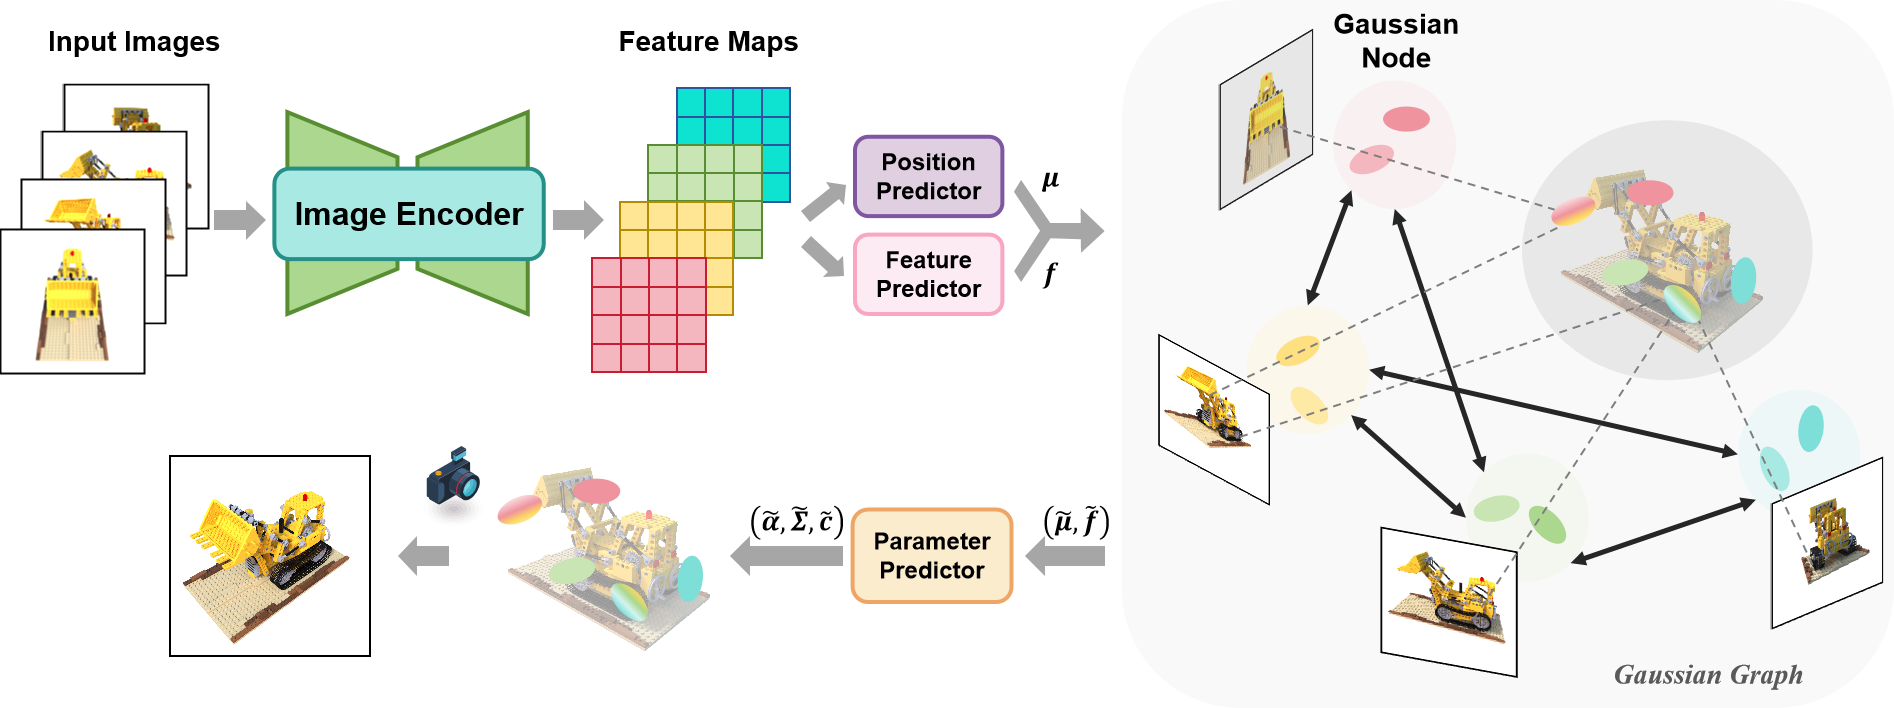
\includegraphics[width=\linewidth]{fig/pipeline.png}
    \caption{Overview of Gaussian Graph Network. Given multiple input images, we extract image features and predict the means and features of pixel-aligned Gaussians. Then, we construct a Gaussian Graph to model the relations between different Gaussian nodes. We introduce Gaussian Graph Network to process our Gaussian Graph. The parameter predictor generates Gaussians parameters from the output Gaussian features. }
    \label{fig:pipeline}
    \vspace{-0.3cm}
\end{figure}
The overall framework is illustrated in Figure~\ref{fig:pipeline}. After predicting positions and features of Gaussian groups from input views with extracted feature maps, we build a Gaussian Graph to model the relations. Then, we process the graph with Gaussian Graph Network via our designed graph operations on Gaussian domain for information exchange and aggregation across Gaussian groups. We leverage the fused Gaussians features to predict other Gaussian parameters, including opacity $\alpha$, covariance matrix $\Sigma$ and colors $c$.

\subsection{Building Gaussian Graphs}

Given $N$ input images $\mathcal{I}=\{I_{i}\}\in\mathbb{R}^{N\times H\times W\times 3}$ and their corresponding camera parameters $\mathcal{C}=\{c_{i}\}$, 
%including intrinsic matrix $c^{I}_{i}\in\mathbb{R}^{3\times 3}$ and extrinsic matrix $c^{E}_{i}\in\mathbb{R}^{4\times 4}$, 
we follow the instructions of pixelSplat~\cite{pixelSplat2023arXiv} and MVSplat~\cite{MVSplat2024arXiv} to extract image features:
\begin{align}
    \mathcal{F}=\Phi_{image}(\mathcal{I}), \quad \mathcal{F}=\{F_{i}\}\in\mathbb{R}^{N\times \frac{H}{4}\times \frac{W}{4}\times C},
\end{align}
where $\Phi_{image}$ is a 2D backbone.
We predict the means and features of pixel-aligned Gaussians:
\begin{align}
    \mu_{i}=\psi_{unproj}\left(\Phi_{depth}(F_{i}), c_{i}\right)\in\mathbb{R}^{HW\times 3}, \quad
    f_{i}=\Phi_{feat}(F_{i})\in\mathbb{R}^{HW\times D}, \label{eq:depth estimation}
\end{align}
where $\Phi_{depth}$ and $\Phi_{feat}$ stand for neural networks to predict depth maps and Gaussian features, and $\psi_{unproj}$ is the unprojection operation.

We build a Gaussian Graph $G$ with nodes $V=\{v_{i}\}=\{(\mu_{i},f_{i})\}_{1\leq i\leq N}$. 
To model the relations between nodes, we define its adjacency matrix $A=[a_{ij}]_{N\times N}$ as:
\begin{equation}
    a_{ij} = 
    \left\{
    \begin{aligned}
       & 1, & i=j \\
       & \psi_{overlap}(v_{i}, v_{j}) , & i\neq j
    \end{aligned}
    \right.
    \label{eq:adjacency matrix}
\end{equation}
where $\psi_{overlap}(v_{i}, v_{j})$ computes the overlap ratio between view $i$ and view $j$.
To limit further computational complexity, we prune the graph by preserving edges with top $n$ weights and ignore other possible edges. 
The degree matrix $D=[d_{ij}]_{N\times N}$ satisfies $d_{ii}=\sum_{j}a_{ij}$. Thus, the scaled adjacency can be formulated as:
\begin{equation}
    \tilde{A}=D^{-1}A \quad \textrm{or} \quad \tilde{A}=D^{-\frac{1}{2}}AD^{-\frac{1}{2}}.
\end{equation}

\subsection{Gaussian Graph Network}

\textbf{Linear Layers.} Assuming that a conventional graph has $N$ nodes with features $\{g_{i}\}\in\mathbb{R}^{N\times C}$ and the scaled adjacency matrix $A=[\tilde{a}_{ij}]_{N\times N}$, the basic linear operation can be formulated as:
\begin{equation}
\hat{g}_{i}=\sum_{j=1}^{N}\tilde{a}_{ij}g_{j}W\in\mathbb{R}^{D},
\end{equation}
where $W\in\mathbb{R}^{C\times D}$ is a learnable weight.
Different from the vector nodes $g_{i}$ in conventional graphs, each node of our Gaussian Graph contains a set of pixel-aligned Gaussians $v_{i}=\{\mu_{i},f_{i}\}$. 
Therefore, we extend the scalar weight $a_{sk}$ of an edge to a matrix $E^{s\rightarrow k}=[e^{s\rightarrow k}_{ij}]_{HW\times HW}$, which depicts the detailed relations at Gaussian-level between $v_{s}$ and $v_{k}$. 
% We define a projection function $\psi_{proj}$:
% \begin{align}
%     \psi_{proj}(\mu,c_{i})=(\mu_{x},\mu_{y}),
% \end{align}
% where $(\mu_{x},\mu_{y})$ is the coordinates of the pixel occupied by $\mu\in\mathbb{R}^{3}$.
For the sake of simplicity, we define
\begin{equation}
    e^{s\rightarrow k}_{ij} = 
    \left\{
    \begin{aligned}
       & 1, & \psi_{proj}(\mu_{s,i}, c_{s})=\psi_{proj}(\mu_{k,j}, c_{s}) \\
       & 0, & \psi_{proj}(\mu_{s,i}, c_{s})\neq\psi_{proj}(\mu_{k,j}, c_{s})
    \end{aligned}
    \right.
    \label{eq:edge matrix}
\end{equation}
where $\mu_{s,i}$ is the center of the $i$-th Gaussian in Gaussian group $v_{s}$, and $\psi_{proj}$ is the projection function which returns coordinates of the occupied pixel. 
% $e^{s\rightarrow k}_{ij}=1$ when the $\mu_{s,i}$ and $\mu_{k,j}$ are projected into the same pixel in the $s$-th view, otherwise $e^{s\rightarrow k}_{ij}=0$.
In this manner, the linear operation on a Gaussian Graph can be defined as:
\begin{equation}
    \hat{f}_{i}=\sum_{j=1}^{N}\tilde{a}_{ij}E^{j\rightarrow i}f_{j}W\in\mathbb{R}^{D}.
\end{equation}
% We employ conventional non-linear operations, such as RELU, GELU, on $\{\hat{f}_{i}\}$. 

\begin{algorithm}[t]
\caption{Gaussian Graph Network}\label{algorithm}
\renewcommand{\algorithmicrequire}{\textbf{Input:}}
\renewcommand{\algorithmicensure}{\textbf{Output:}}
\begin{algorithmic}
\Require Multi-view images $\mathcal{I}=\{I_{i}\}$, camera parameters $\mathcal{C}=\{c_{i}\}$, the number of graph layers $h$
\Ensure Gaussian parameters $(\mu, \Sigma, \alpha, c)$
\State $\mathcal{F}\leftarrow\Phi_{image}(\mathcal{I}, \mathcal{C})$

\State $\mu_{i}\leftarrow\psi_{unproj}\left(\Phi_{depth}(F_{i}), c_{i}\right), \quad
    f_{i}\leftarrow\Phi_{feat}(F_{i})\quad i=1,2,\cdots,N$

\State $\tilde{A}\leftarrow D^{-1}A$
\For{$k\leftarrow 1$ to $h$}
    \State $f_{i}\leftarrow\sigma\left(\sum\tilde{a}_{ij}E^{j\rightarrow i}f_{j}W\right)\quad i=1,2,\cdots,N$
\EndFor
% \State Search connected components $\{G^{s}\}_{1\leq s\leq l}$
\State $(\mu, f)\leftarrow\bigcup_{s=1}^{l}\phi_{pooling}(G^{s})$
\State $R, S, \alpha, c\leftarrow\psi_R(f),\psi_S(f),\psi_{\alpha}(f),\psi_{c}(f)$
\State $\Sigma\leftarrow RSS^{\top}R^{\top}$
\end{algorithmic}
\end{algorithm}

\textbf{Pooling layers.} If we have a series of connected Gaussian Graphs $\{G^{s}\}_{1\leq s\leq l}$, where $G^{s}\subseteq G$, then we operate the specific pooling operation on each $G^{s}$ and combine them together:
\begin{equation}
    \phi_{pooling}(G)=\bigcup_{s=1}^{l}\phi_{pooling}(G^{s}).
\end{equation}
If $G^{s}$ only contains one node $v^{s}$, $\phi_{pooling}(G^{s})=v^{s}$.
Otherwise, we start with a random selected node $v_{i}^{s}=(\mu_{i}^{s},f_{i}^{s})\in G^{s}$. 
Since $G^{s}$ is a connected graph, we can randomly pick up its neighbor $v_{j}^{s}$ with corresponding camera parameters $c_{j}^{s}$.
% We define a function $\psi_{similarity}$ to measure the similarity:
% \begin{equation}
%     \psi_{similarity}\left(v_{j,m}^{s}, v_{i}^{s}\right)=\max_{n} \gamma_1\dfrac{f^{s}_{j,m}\cdot f_{i,n}^{s}}{\Vert f^{s}_{j,m}\Vert\Vert f_{i,n}^{s}\Vert} - \gamma_2\|\mu^{s}_{j,m}-\mu_{i,n}^{s}\|,
% \end{equation}
% where $\gamma_1$ and $\gamma_2$ are hyperparameters, and $v_{j,m}^{s}=(\mu^{s}_{j,m},f^{s}_{j,m})$ is a Gaussian in node $v_{j}^{s}$.
We define a function $\psi_{similarity}$:
\begin{equation}
    \psi_{similarity}\left(v_{j,m}^{s}, v_{i}^{s}\right)=
    \begin{cases}
        \mathop{\max}\limits_{n}\Vert\mu_{j,m}^{s}-\mu_{i,n}^{s}\Vert, & \mathop{\max}\limits_{n} e_{mn}^{j\rightarrow i}=1 \\
        \infty, & \mathop{\max}\limits_{n} e_{mn}^{j\rightarrow i}=0
    \end{cases} 
\end{equation}
where $v_{j,m}^{s}$ is the $m$-th Gaussian in node $v_{j}^{s}$. We define the merge function $\psi_{merge}$:
\begin{equation}
    \psi_{merge}\left(v_{j,m}^{s}, v_{i}^{s}\right)=
    \begin{cases}
        \varnothing, & \psi_{similarity}\left(v_{j,m}^{s}, v_{i}^{s}\right)<\lambda\\
        v_{j,m}^{s}, & \textrm{otherwise}
    \end{cases}
\end{equation}
Then, we merge two nodes together to get a new node
\begin{equation}
    v_{new}^{s}=\bigcup_{m=1}^{HW}\psi_{merge}\left(v_{j,m}^{s}, v_{i}^{s}\right)\cup v_{i}^{s}
\end{equation}
In this manner, we aggregate a connected graph $G^{s}$ step by step to one node. Specifically, previous methods can be considered as a degraded Gaussian Graph without edges:
\begin{equation}
    \phi_{pooling}(G)=\bigcup_{s=1}^{N}\phi_{pooling}(G^{s})=\bigcup_{s=1}^{N}v^{s}.
\end{equation}
where $\phi_{pooling}$ degenerates to simple combination of nodes.

\textbf{Parameter prediction.} After aggregating the Gaussian Graph $(\mu,f)=\psi_{pooling}(G)$, we predict the rotation matrix $R$, scale matrix $S$, opacity $\alpha$ and color $c$:
\begin{equation}
    R=\phi_{R}(f),\quad S=\phi_{S}(f),\quad \alpha=\phi_{\alpha}(f), \quad c=\phi_{c}(f)
\end{equation}
where $\phi_{R}$, $\phi_{S}$, $\phi_{\alpha}$ and $\phi_c$ are prediction heads. The covariance matrix can be formulated as:
\begin{equation}
    \Sigma=RSS^\top R^\top.
\end{equation}
 Our Gaussian Graph Network is illustrated in Algorithm~\ref{algorithm}, where $\sigma$ stands for non-linear operations, such as ReLU and GeLU.










 


